% This LaTeX was auto-generated from an M-file by MATLAB.
% To make changes, update the M-file and republish this document.

\documentclass[12pt]{article}
\usepackage{natbib}
\usepackage[french]{babel}
\usepackage[utf8x]{inputenc}
\usepackage{lipsum}
\usepackage{amsmath}
\usepackage{graphicx}
\usepackage[final]{pdfpages}
\usepackage[T1]{fontenc}
%\usepackage[colorinlistoftodos]{todonotes}
\usepackage{xcolor}
\usepackage[nottoc,numbib]{tocbibind}% Para que la bibliografia salga en el table of contents
\colorlet{Mycolor1}{green!10!orange!90!}
\usepackage{subfigure}
\sloppy
\definecolor{lightgray}{gray}{0.5}
\setlength{\parindent}{0pt}
\setlength{\parskip}{1em}

\bibliographystyle{abbrv}

\begin{document}
\title{Compte rendu Initiation a la recherche}
\author{CHIRINO CAICEDO Melet \and RIBEIRO GOMES Bruno}
\begin{titlepage}

\newcommand{\HRule}{\rule{\linewidth}{0.5mm}} % Defines a new command for the horizontal lines, change thickness here

\center % Center everything on the page
 
%----------------------------------------------------------------------------------------
%	HEADING SECTIONS
%----------------------------------------------------------------------------------------

\textsc{\LARGE Université Toulouse III}\\[0.5cm] % Name of your university/college
\textsc{\Large Paul Sabatier}\\[1.0cm] % Major heading such as course name
\textsc{\large Rapport du stage 2020/2021}\\[0.5cm] % Minor heading such as course title

%----------------------------------------------------------------------------------------
%	TITLE SECTION
%----------------------------------------------------------------------------------------

\HRule \\[0.4cm]
{ \huge \bfseries Projet Linky4Teens}\\[0.4cm] % Title of your document
\HRule \\[1.5cm]
 
%----------------------------------------------------------------------------------------
%	AUTHOR SECTION
%----------------------------------------------------------------------------------------

\begin{minipage}{0.4\textwidth}
\begin{flushleft} \large
\markboth{Pojet en \LaTeX}
\emph{Auteurs:}\\
\textsc{CHIRINO} Melet \\ % Your name
%\textsc{RIBEIRO} Bruno % Your name
\end{flushleft}
\end{minipage}
~
\begin{minipage}{0.5\textwidth}
\begin{flushright} \large
\emph{Tuteur:} \\
\textsc{RIVIERE} Nicolas  % Supervisor's Name
\end{flushright}
\end{minipage}\\[2cm]

% If you don't want a supervisor, uncomment the two lines below and remove the section above
%\Large \emph{Author:}\\
%John \textsc{Smith}\\[3cm] % Your name

%----------------------------------------------------------------------------------------
%	DATE SECTION
%----------------------------------------------------------------------------------------

{\large \today}\\[2cm] % Date, change the \today to a set date if you want to be precise

%----------------------------------------------------------------------------------------
%	LOGO SECTION
%----------------------------------------------------------------------------------------


\includegraphics[width=6in]{img/Logo_UT3.jpg}\\[2cm] % Include a department/university logo - this will require the graphicx package
 
%----------------------------------------------------------------------------------------

\vfill % Fill the rest of the page with whitespace

\end{titlepage}

%\{Contents}
\tableofcontents

\newpage

%-------------------------- * Introduccion * --------------------------------

\section{Introduction}
%Aqui explico de que se trata el proyecto y lo que habiamos hecho antes como TER
El proyecto linky4teens es un proyecto que busca desarrollar prototipos que ayuden a mejorar el desempenho en atletas jovenes llevado por el club Balma y el Profesor Yann LABIT. El proyecto busca crear dispositivos para revisar el desempenho de los atletas y trabajar sobre los errores que se esten cometiendo. 

Yo estaba encargado de seguir el desarrollo de dos prototipos desarrollados en proyectos anteriores como proyectos de TER:
\begin{itemize}
    \item Temoin de relevos inteligente (desarrollado por mi un grupo de amigos)
    \item Starting block
\end{itemize}
Estos proyectos al estar financiados por estudiantes estaban bien pero necesitaban mejoras y mucha robustez para funcionar como producto funcional.

%-------------------------- * Desbcripcion * --------------------------------

\section{Bref description du systeme}
Aqui vas a mostrar unos cuantos diagramitas UML para explicar como funcionan las cosas dentro tus chocoros

%-------------------------- * Objetivos * --------------------------------

\section{Objectifs}
Los objetivos de stage eran rendre plus robuste los prototipos ya existentes y/o los sistemas creados.
\begin{itemize}
    \item Mejorar el dock
    \item Mejorar los temoins
    \item Mejorar la interfaz
    \item Mejorar el Starting block e integrarlo a una unica interfaz de proyecto
\end{itemize}
\section{Mejoras propuestas}
\begin{itemize}
    \item Dock: utilisar una raspberry pi como dock porque esta puede usar conexion wifi direct a cualquier dispositivo que pueda acceder a internet sin necesidad de instalar porgramas o aplicaciones. 
    \item Temoin: el temoin estaba soldado en una pcb universal y era muy endeble, habia que volverlo mas robusto y, el punto mas importante, no guardaba suficiente informacion, por lo tanto las mediciones eran medio jopos. Ademas el sistema de barreras IR era poco robusto. Todo eso debia mejorarlo.
    \item Interfaz: la interfaz utilisaba un deploy de django (un framework web escrito en python porque? porque yo lo se usar, asi de simple). Pero estaba muy simple por propias limitaciones del sistema pero con mas financiacion se podia mejorar todo.
    \item Starting block: conectarlo por wifi a la interfaz para que se pueda mejar desde ahi de manera practica y sencilla. A peticion del club una base de datos no quedaria nada mal para organizar la informacion.
\end{itemize}

%-------------------------- * Obligaciones administrativas * --------------------------------
\section{Obligaciones Administrativas}
Al ser un proyecto financiado por la fac tenia ciertas obligaciones administrativas como enviarle poticiones al tecnincien encharge jerome raybayrol para hacer los debis y pedir los componenetes. Ademas se me suministraron herramientas como un osciloscopio y un taladro para poder trabajar a distancia (tu sabes esto de la situacion del mundo y tales)
%-------------------------- * Obligaciones Tecnicas * --------------------------------
\section{Obligaciones Tecnicas}
Este proyecto tuvo muchas cosas desarrolladas en computador y muchisima programacion. Sin embargo tambie tuve mucha accion en el fablab de la fac para fabricar piezas en la impresora 3d, la cortadora laser y la maquina cnc para hacer unos circuitos.
\subsection{Logiciels de CAO}
Los logiciel de CAO son muy importantes, para fabricar los circuitos, simularlos y disenhar su fabricacion. Como logiciel utilise Eagle (tambien porque era el que sabia usar). 
\begin{figure}[!htb]
\centering
\subfigure[PCB du circuit]{\includegraphics [height=2in]{img/EagleBoard.png}
\label{img:eagle:board}}
\subfigure[Schema du circuit]{\includegraphics [height=2in]{img/EagleSchema.png}
\label{img:eagle:schema}}
\caption{Captures d'Eagle}
\end{figure}
Para los dispositivos 3D utilise la plataforma online OnShape la cual es gratuita y tambien permita compartir los disenhos en 3D con todos los participantes del proyecto (si solo hubiera mas gente) y tambien gestionar las versiones. sur la bibliographie vous trouverez le repo avec les fichiers
\begin{figure}[!htb]
\centering
\subfigure[Conception de la Barriere IR]{\includegraphics [height=2in]{img/OnShapeBarriere.png}
\label{img:onshape:barriere}}
\subfigure[Boite du starting block]{\includegraphics [height=2in]{img/OnShapeSB.png}
\label{img:onshape:sb}}
\subfigure[Conception mecanique du temoin]{\includegraphics [width=2.7in]{img/OnShapeTemoin.png}
\label{img:onshape:temoin}}
\caption{OnShape}
\end{figure}
%Aqui coloca imagenes del repo asi como la url del repo
\subsection{Service electronique de Paul Sabatier}
Para fabricar circuitos alguien me informo que puedo acceder al servicio de fabricacion electronica de la universidad, tuve que ponerme en contacto con el senhor guillaume Maffre quien me gui por el proceso. A mediados del mes de mayo cambiaron el proceso de metalizacion y al parecer no era tan efectivo como el anterior porque varios circuitos no tenian bien la metalizacion, es el proceso que conecta la capa de arriba con la de abajo. Ademas este proceso tomaba de 3 dias a una semana dependiando de la complejidad del pcb. Por lo cual decidi no usar este servicio a menos que fuera estrictamente necesario.

\subsection{Manufactura con herramientas de fablab}
El hecho de trabajar con hardware requiere muchas herramientas y espacio para trabajar, lo cual no tengo en casa. GraciajaDios la fac cuenta con el fablab del cual soy abone y me puedo en servir de todas sus herramientas y maquinas.

La primera herramienta que use fue la maquina cnc para fabricar unas pcb pequenhas. Este proceso lo hice con la ayuda del logiciel flatCAM y un simulador de maquinas cnc porque con la situacion sanitaria tenia que priorizar al maximo el teletrabajo.

\begin{figure}[!htb]
\centering
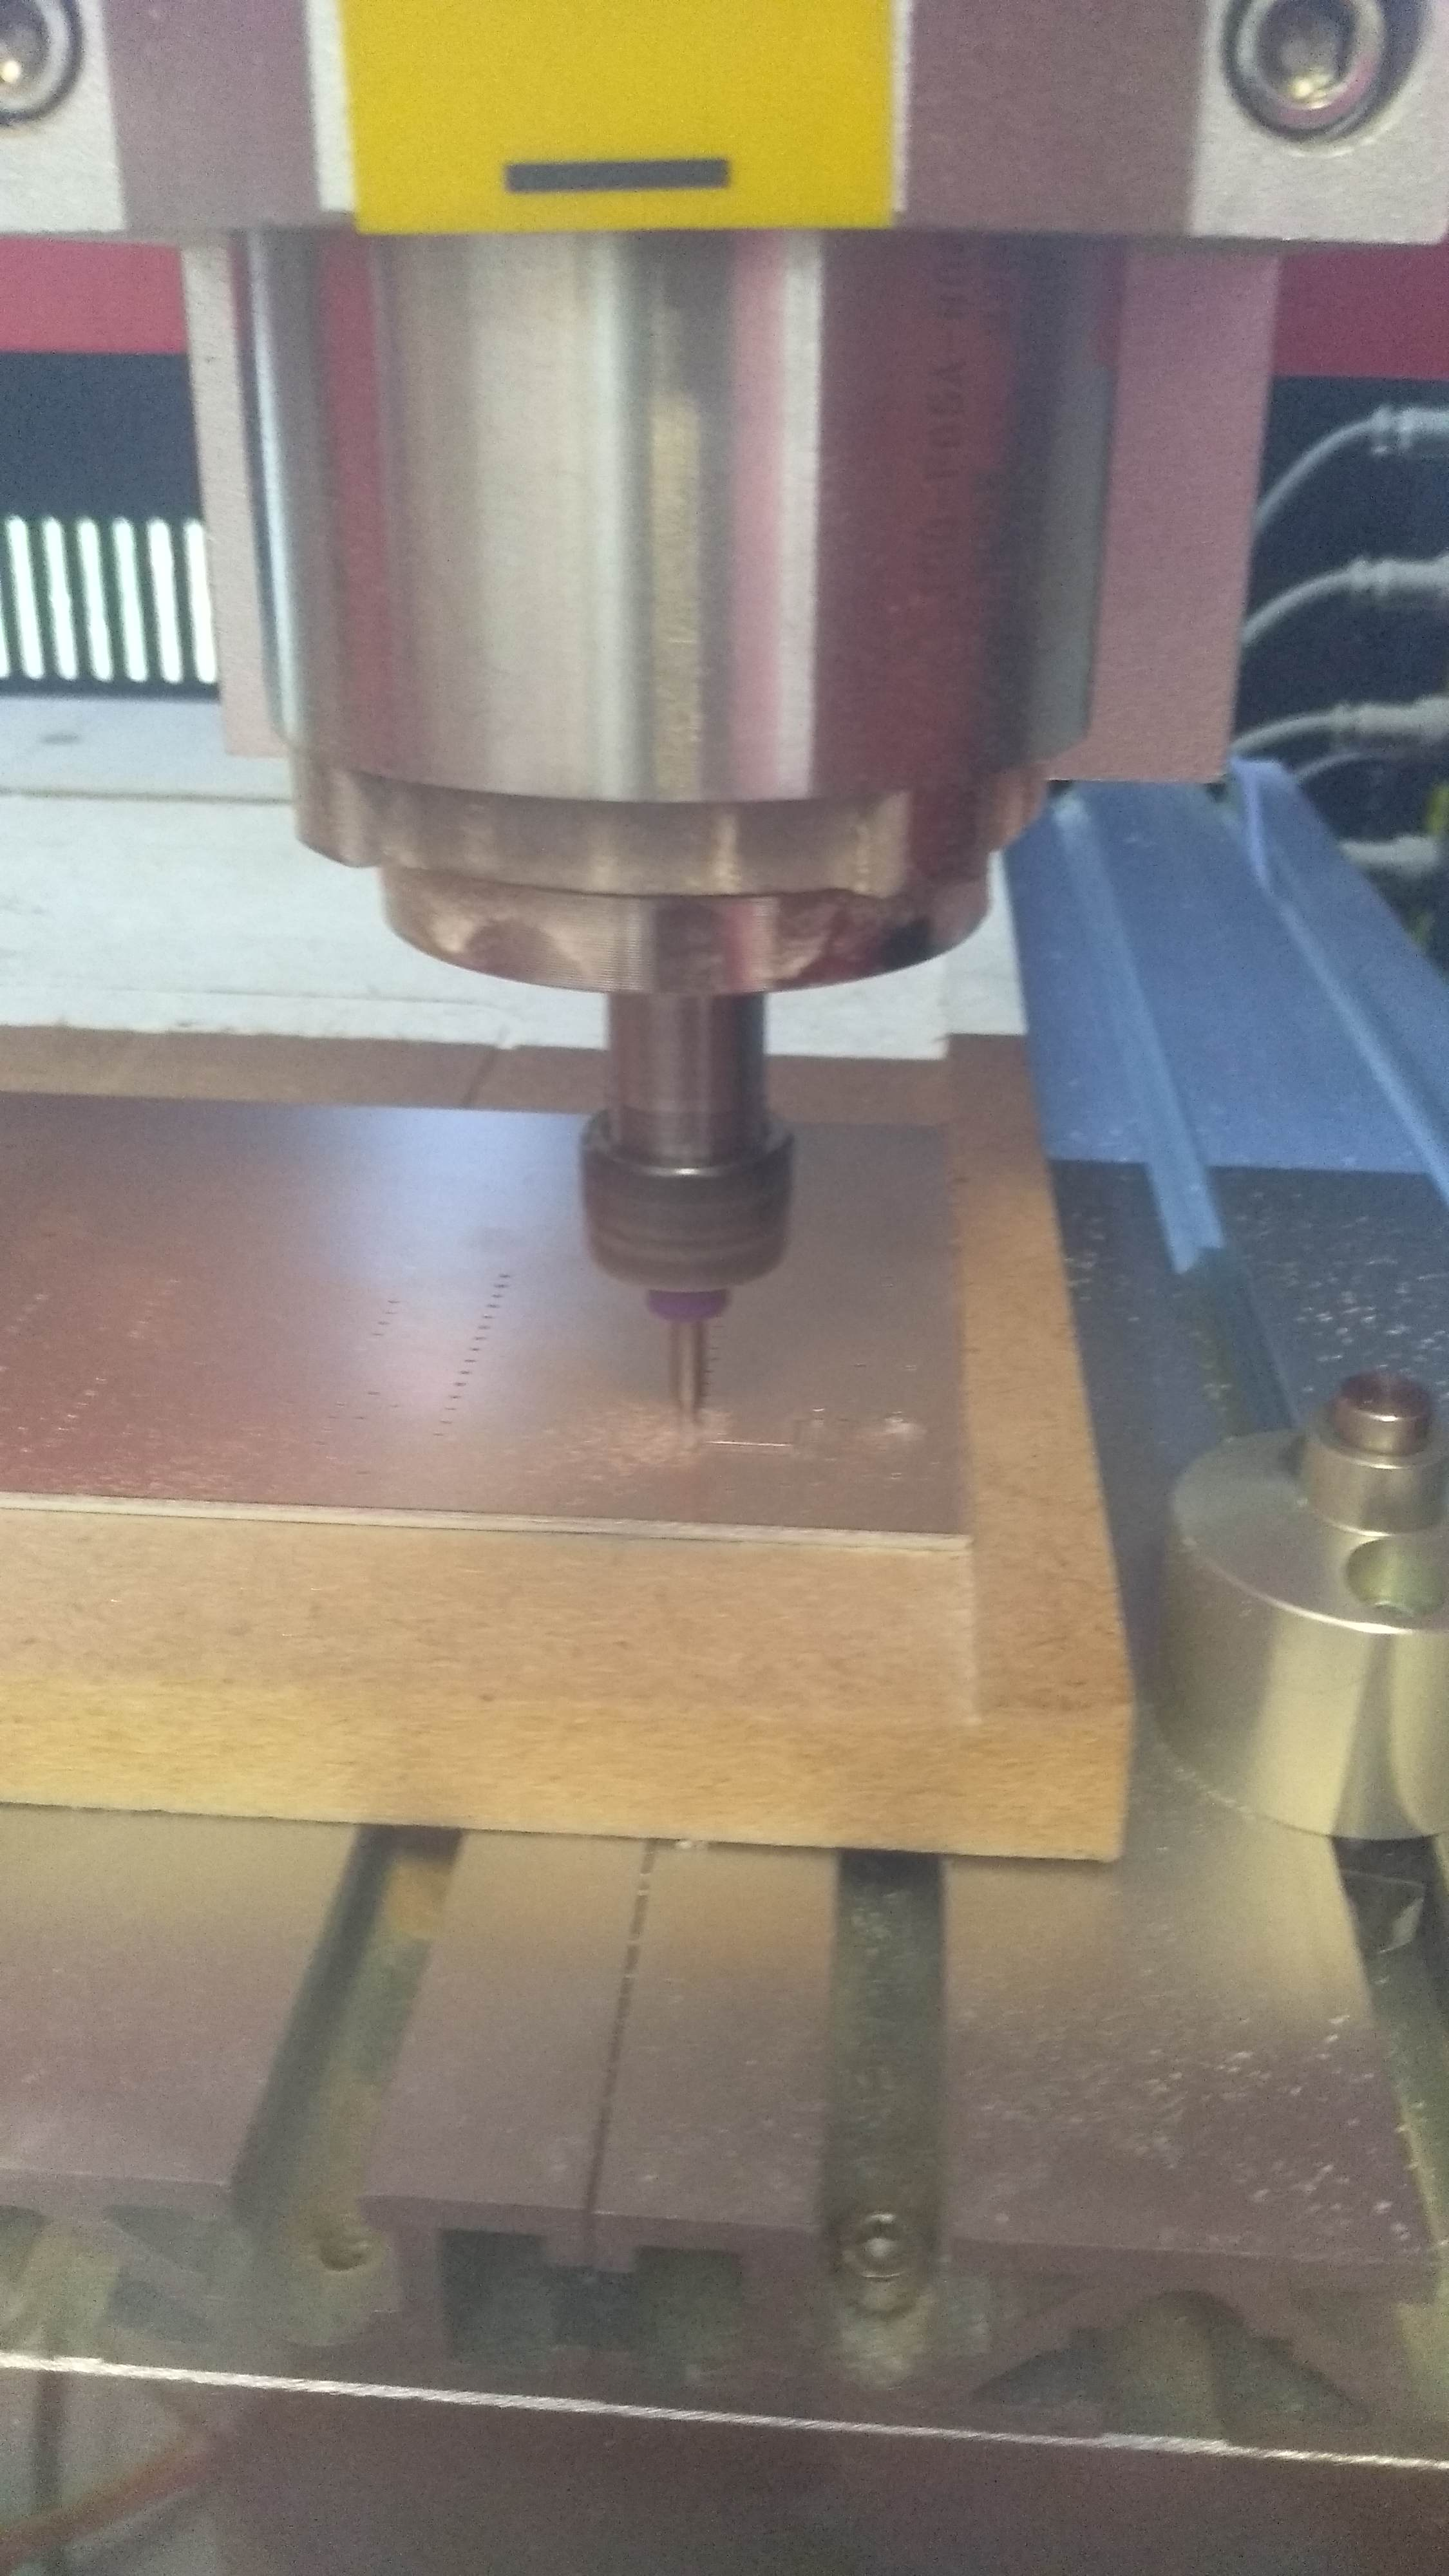
\includegraphics[width=0.2\textwidth]{img/CNCRouter.jpg}
\caption{Machine CNC pour le routage des PCB}
\label{img:RouterCNC}
\end{figure}

\begin{figure}[!htb]
\centering
\includegraphics[width=0.2\textwidth]{img/FlatCAM.png}
\caption{Logiciel pour le routage des PCB}
\label{img:flatcam}
\end{figure}

Luego de hacer los circuitos utilice la estacion de soldadura para montarlos componentes en la pcb.

\begin{figure}[!htb]
\centering
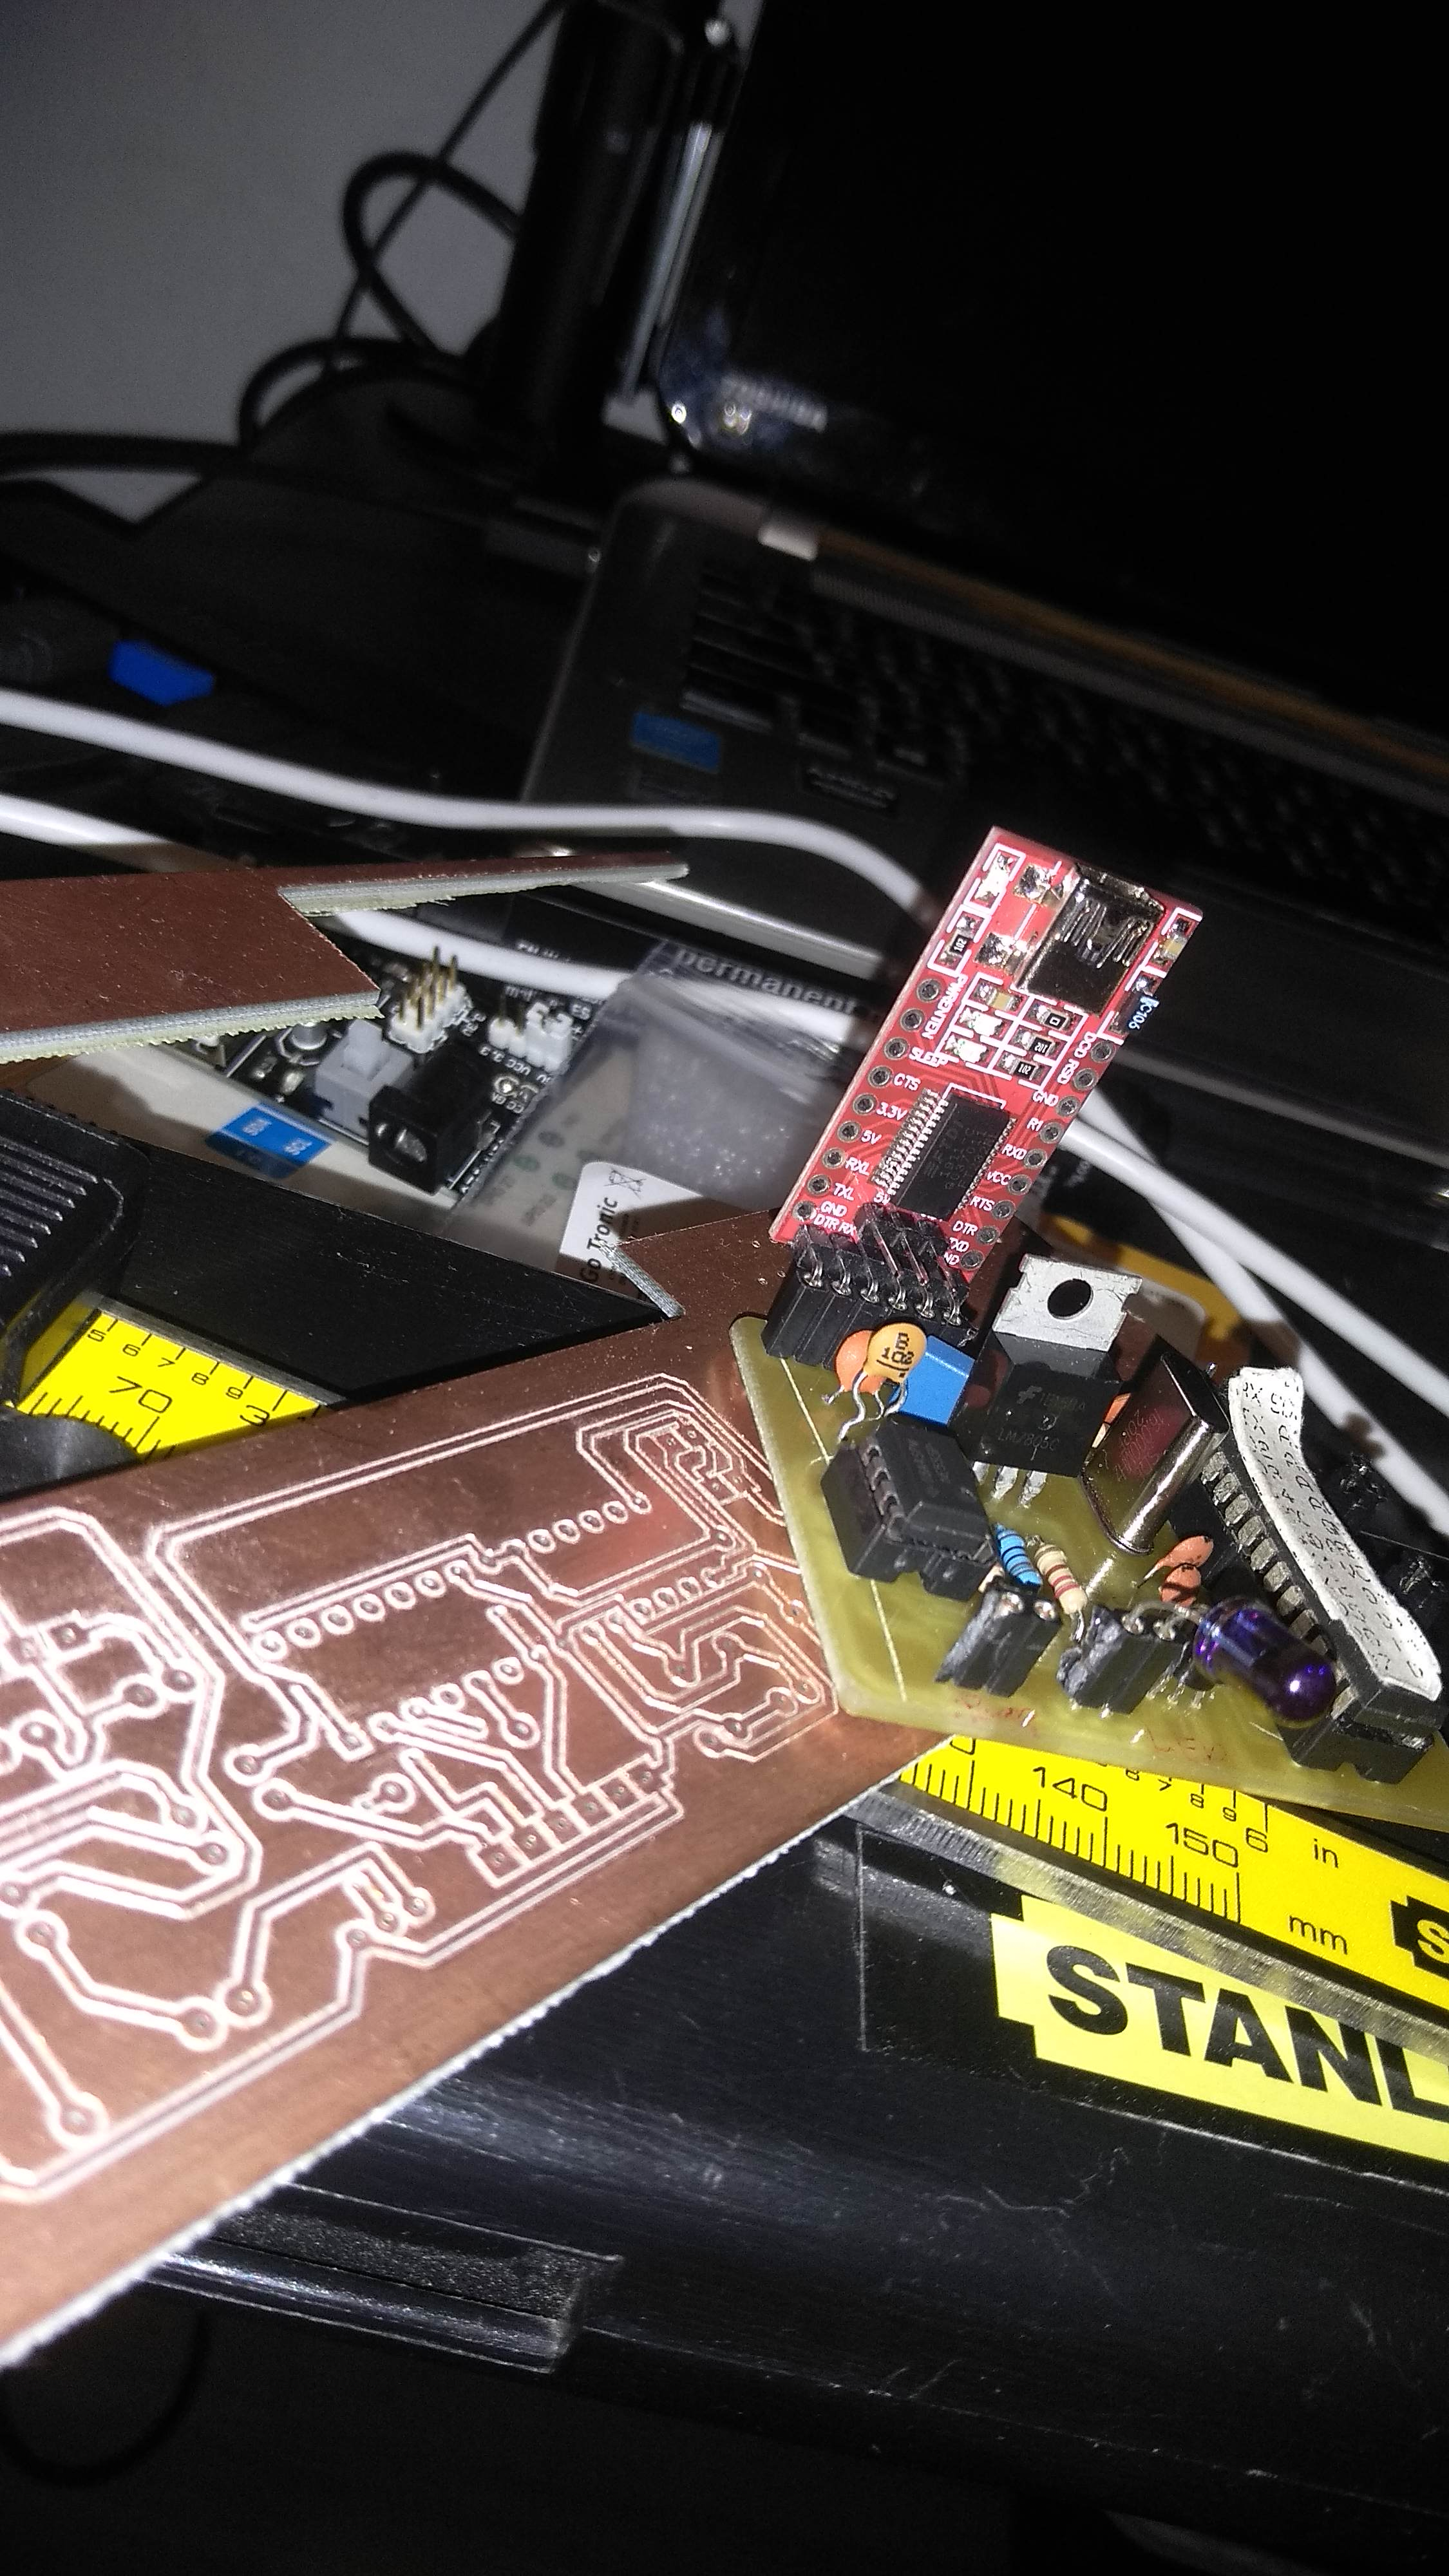
\includegraphics[width=0.2\textwidth]{img/CircuitosCNCed.jpg}
\caption{Des circuits apres le CNC Router}
\label{img:CircuitsCNCd}
\end{figure}
La ultima herramienta que utilise fue la cortadora laser para hacer el soporte de las barieres IR y la nueva cajita del starting block (mas pequenha y tales)

La impresora 3D tenia pensado usarla para hacer el temoin en PLA transparente y estuve imprimiento un cable chain para mejorar la robustez de los cables en el starting block.

\begin{figure}[!htb]
\centering
\subfigure[Decoupe Laser]{\includegraphics [height=2in]{img/CortadoraLaser.png}
\label{img:LaserCutter}}
\subfigure[Premiere essaye du Barriere IR]{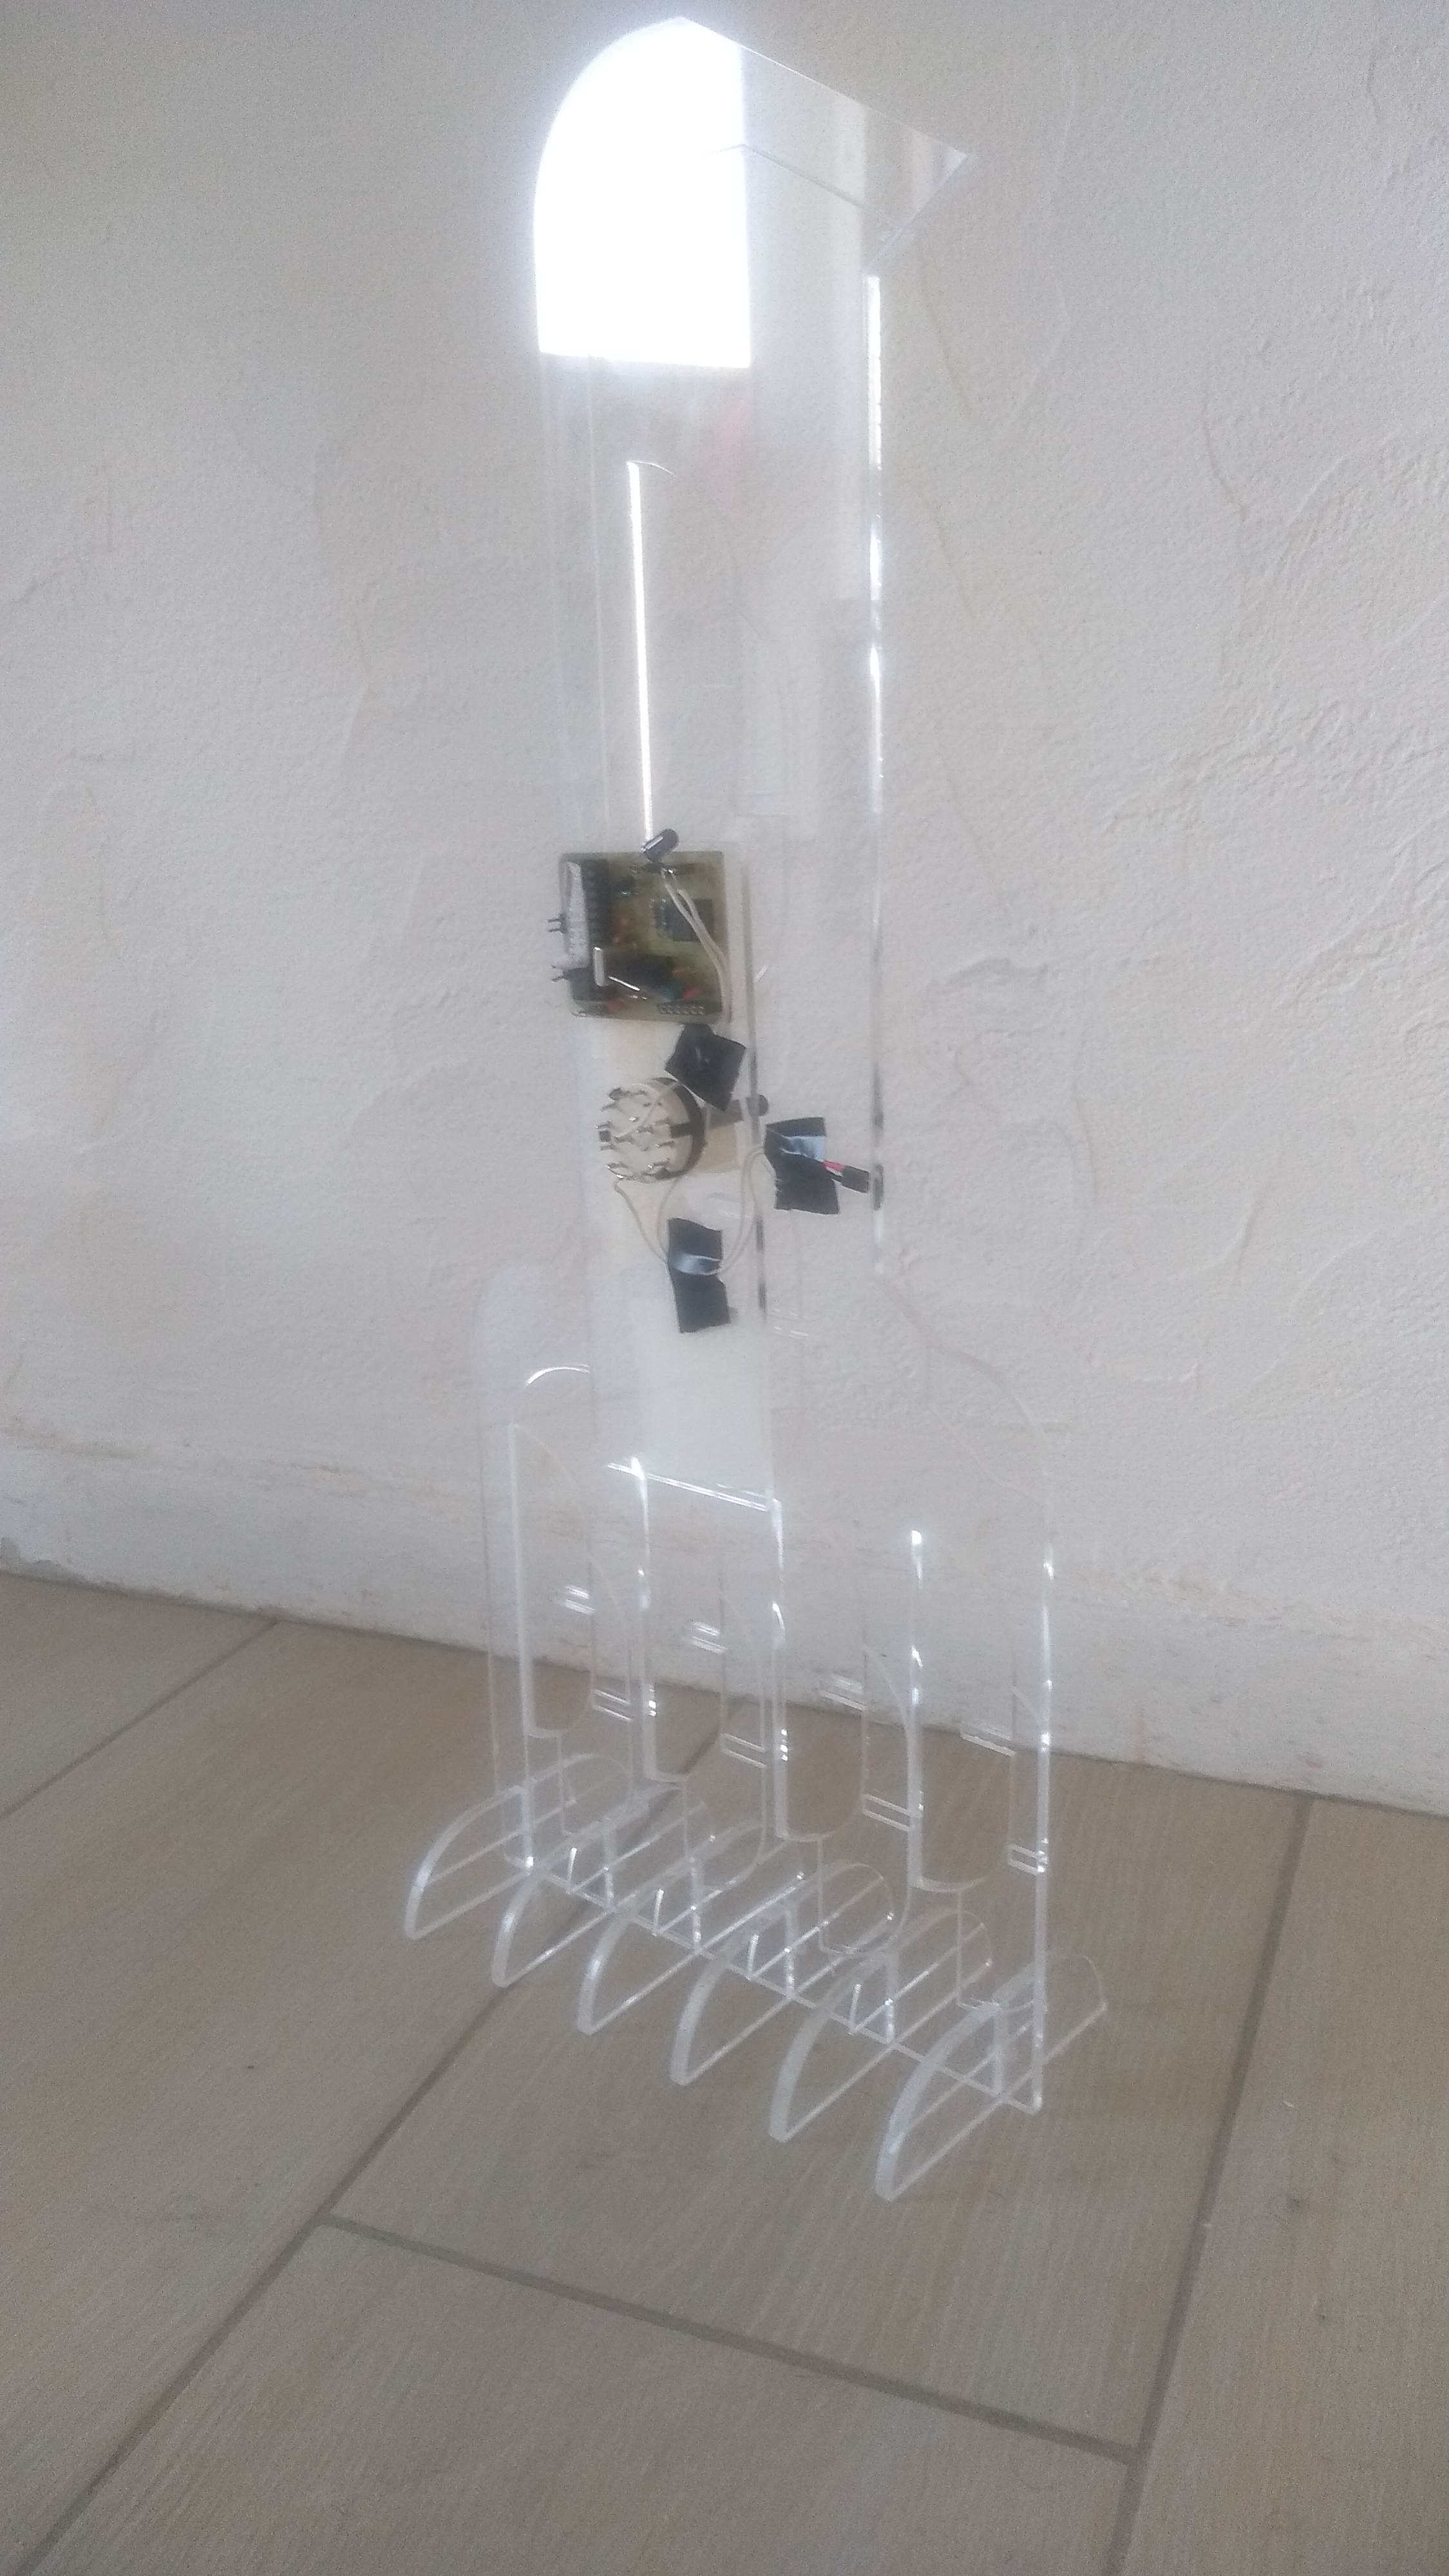
\includegraphics [height=2in]{img/BarriereIrV1.jpg}
\label{img:BarriereV1}}
\caption{Resultats de la decoupe laser}
\end{figure}

El resto de herramientas miscelaneas, el gran espacio y la gente con experiencia en hardware creo un ambiente muy chevre para trabajar en grupo

\subsection{Utilisation de github como gestor de proyecto}
Al ser un proyecto donde mas de la mitad del trabajo es programacion es necesario tener un gestor de versiones para el cual utilise git. Ademas Github es excelente como herramienta de gestion compartida.

Otra ventaja de github es que ofrece una pagina de wikis donde se puede dejar toda la documentacion por si alguien retoma el proyecto donde yo lo estoy dejando ahora mismo. Tambien tiene la seccion de gestion de proyectos que es parecida a slack donde pongo lo que voy haciendo poco a poco y el tutor de stage puede revisar mi trabajo poco a poco. 

La seccion de issues tambien es buenisima para el trabajo en grupo y si alguien a futuro tiene problemas con mi proyecto yo puedo ayudarlo a solucionar el problema.
\begin{figure}[!htb]
\centering
\subfigure[Repositoire sur github]{\includegraphics [height=2in]{img/Repo.png}
\label{img:git:repo}}
\subfigure[Outil de gestion de projets de github]{\includegraphics [height=2in]{img/GithubProject.png}
\label{img:git:project}}
\subfigure[Wikis sur github]{\includegraphics [width=2.7in]{img/GitWiki2.png}
\label{img:git:wiki}}
\caption{Images du repo}
\end{figure}

%-------------------------- * Seccion de resultados * --------------------------------

\section{Resultados}
Los resultados se vieron afectados por varios factores ajenos al desarrollo del proyecto como mi rattrapage a mitad de junio, varias pcb que vinieron malas y faltando dos semanas para terminar el stage me dio covid y cuando pude salir el fablab estaba cerrado y solo me faltaba terminar de fabricar las piezas del temoin. Para colmo se quemaron 2 step up y no pude nisiquiera pude soldar los temoin (y habia uno que tenia unos vias que no hacian conexion, maldita sea). A pesar de todo eso pude avanzar mucho en otras cosas.

%-------------------

\subsection{Raspberry como dock multifuncional}
La raspberry como dock multifuncional es le mejor avance que hice ya que ahora tiene una base de datos que permite ingresar atletas, coachs y llevar un historal de todas las sesiones de entrenamiento. Ademas se conecta directamente al starting block y permite ver su estado de bateria. 
Tambien permite actualizar la interfaz directamente desde github, lo que permitiria venderlo como producto y actualizarlo con el pasar del tiempo.
Toda la informacion guardada es ademas exportable por si se quiere hacer un tratamiento de datos externo.
\begin{figure}[!htb]
\centering
\includegraphics[width=0.4\textwidth]{img/LandingPage.png}
\caption{Page d'accueil}
\label{img:gui:landing-page}
\end{figure}
\begin{figure}[!htb]
\centering
\includegraphics[width=0.4\textwidth]{img/SessionDetail.png}
\caption{Detail de chaque seance du sport}
\label{img:gui:session-detail}
\end{figure}
\begin{figure}[!htb]
\centering
\includegraphics[width=0.4\textwidth]{img/SessionList.png}
\caption{Liste de toutes les seances du sports enregistr\'es}
\label{img:gui:session-list}
\end{figure}
\subsection*{Mejoras}
Como mejora esta meterle una bateria y que esta cargue los temoins. Mostrar tambien la carga del propio aparato. y terminar la parte que se conecta con el temoin, la cual esta testeada con datos simulados que funcionan bien.
Otra mejora que tengo pensado ponerle es una opcion que permita un calibrage automatico de los sensores de fuerza para no tener que desarmar el dispositivo cada vez que se descalibre.

%-------------------

\subsection{Startingblock 2.0}
El mayo cambio en el starting block en terminos de harwdware es su tamanho mas reducido y el uso de una bateria de ion de litio recargable directamente desde la cajita. Segun las pruebas de rendimiento el dispositivo consume aproximadamente unos 100mA de corriente de forma constante con pequenhos picos de corriente de 200mA por lo cual se puede estimar la duracion de la bateria. (aqui pones fotos del videito que grabaste)
\begin{figure}[!htb]
\centering
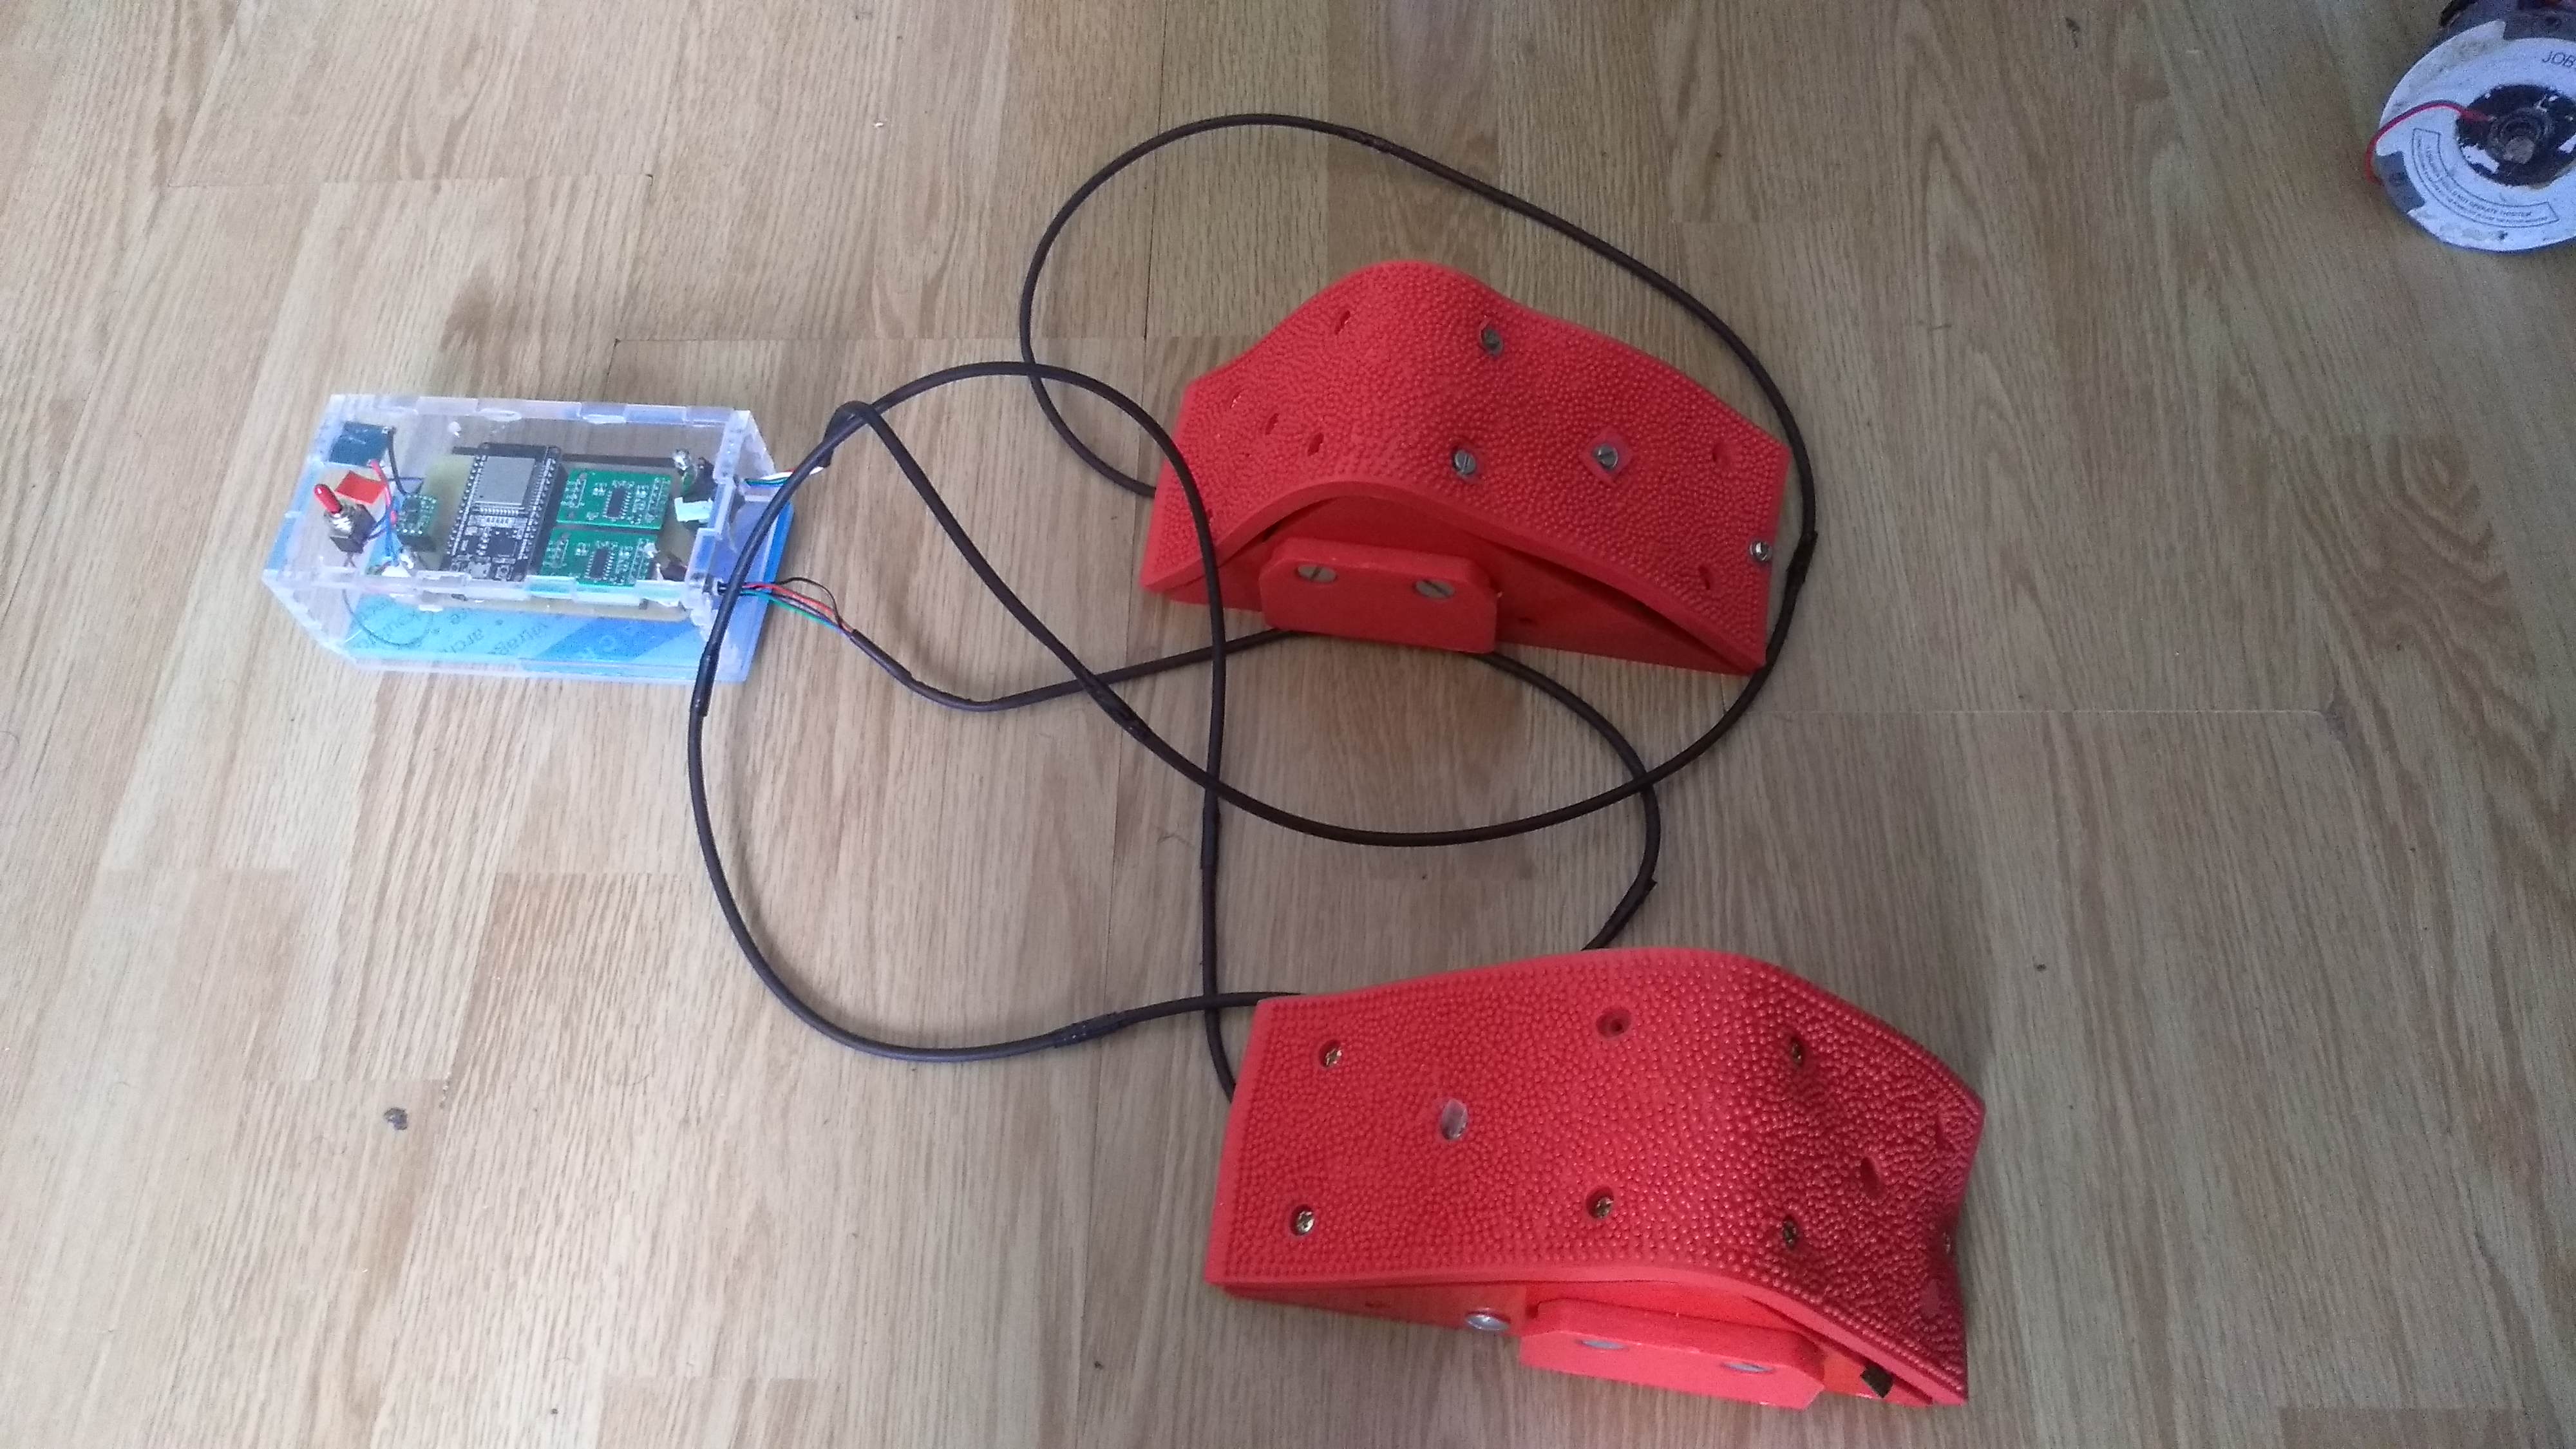
\includegraphics[width=0.5\textwidth]{img/StartingBlockCompleto.jpg}
\caption{Starting Block}
\label{img:sb:complete}
\end{figure}
\subsection*{Mejoras}
Agregarle a la programacion el programa de calibracion (el cual ya viene listo en la libreria de los amplificadores) que se haga directamente desde la interfaz grafica.

Otra cosa que no tuve en cuenta es el disenho que favorezca un depanage. Actualmente es muy complicado desarmar todo para revisar si algo falla, eso fue un error de disenho que no tuve en cuenta.
Una ultima mejora es agregarle un capacitor que ayude a la bateria en los picos de corriente para aumentar la vida util de la bateria.

%-------------------

\subsection{Mejoras para los temoin}
Los temoin y las barrieres IR tuvieron una mejora sustancial en terminos de usabilidad y componentes. Lastima que las pcb del protipo final vinieron con fallas y no se pudo armar un dispositivo final, ademas que habian unos step up que se quemaron y solo me quedaba uno y lo use para el starting block que ya estaba armado para tener una cosa que sirviera. Ademas de todo esto, la imposibilidad de ir al fablab la ultima semana me limito mucho porque tuve covid y aja eso me cago la vida.
\subsection*{Mejoras}
Basicamente falta armarlos y probarlos, ahi falle pero me perjudico la situacion sanitaria ya que esta semana tenia pensado hacer esas cosas.

%-------------------

\subsection{Documentacion del proyecto}
La documentacion actual es la de la version del poryecto TER y me falta agregarle todas las cosas que desarrolle hasta este momento. Viendo que utilise un framework web y que no todo el mundo sera capaz de utilizar este framework intente factorizar las funciones al maximo para que cualquier pueda modificar las funciones que hacen las cosas importantes sin tener que meterse directamente con el framework.
Para documentar tambien utilise doxygen que genero un archivo pdf con la explicacion de todas las funciones en C.
\begin{figure}[!htb]
\centering
\includegraphics[width=0.5\textwidth]{img/GitWiki.png}
\caption{Wikis du Github}
\label{img:git:wikis1}
\end{figure}
\subsection*{Mejoras}
Me encantaria documentar todo el framework de django pero es un trabajo largo y duro, asi que lo dejo como trabajo futuro.

%\begin{figure}[!htb]
%\centering
%\includegraphics[width=0.2\textwidth]{images/ubication-sipi.png}
%\caption{Location du village Sipí \cite{sipi:ubicacion}}
%\label{img:sipi:ubicacion}
%\end{figure}

% Plantilla para colocar muchas imagenes con un multiplot
%\begin{figure}[!htb]
%\centering
%\subfigure[Photo trouv\'e sur Facebook]{\includegraphics %[height=2in]{images/image18.png}
%\label{img:sipi-urbana}}
%\subfigure[Photo prise par la mairie de Sip\'i ]{\includegraphics %[height=2in]{images/alcaldia-sipi.jpg}
%\label{img:sipi-urbana2}}
%\subfigure[Photo pris par le quotidien Colombien \textit{CNC Noticias}]{\includegraphics %[width=2.7in]{images/image39.png}
%\label{img:sipi-urbana3}}
%\caption{Images de Sip\'i}
%\end{figure}
%Sur la Figure \ref{img:sipi:boats} on peut voir les bateaux transportant des personnes et des biens.



%Para citar la bibliografia haces \cite{Photovoltaic}
%Para referenciar las imagenes haces lo sgte \ref{fig:schema}


\section{Conclusion}
Este stage fue muy interesante y aprendi muchas cosas como gestionar un proyecto, usar diferentes logiciels para plantear las cosas e incluso utilise plantuml para planear las cosas pero no funciono del todo, cagada eso. Aprendi mucho y estuvo bueno todo mientras duro.
%debes hacer esto para meter archivos de otro lado
%\input{sub_files/Calcul_puissance}
%\label{anexe:calcul-puissance}
%-------------------

%Para meter un pdf haces lo sgte 
%\includepdf{images/Velocidad-Maxima-Energia_13}
%\label{pdf:vent_vitesse_max}
%-------------------

% \begin{figure}
%     \centering
%     \includegraphics[height=\textheight]{Anexes/RadiacionSolar13 (1).pdf}
%     \caption{Caption}
%     \label{fig:radiacion}
% \end{figure}


% Plantilla para colocar muchas imagenes con un multiplot
%\begin{figure}[!htb]
%\centering
%\subfigure[]{\includegraphics [width=2.5in]{lab_2_vision_15.png}}
%\subfigure[]{\includegraphics [width=2.5in]{lab_2_vision_16.png}}
%\subfigure[]{\includegraphics [width=2.5in]{lab_2_vision_17.png}}
%\caption{Paleta de colores}
%\end{figure}

% Plantilla para poner una imagen cualquiera
%\begin{figure}[!htb]
%\centering
%
%\caption{Histograma de la imagen}
%\end{figure}

%\bibliography{Biblio}

\end{document}